\section{Buffer overflow with sign detection} \label{sec:exercise3}
Buffer overflow is historically one of the most common programming errors. It is the cause of security breaches, data corruption and program crashes. Detecting them is therefore preferred.
\\\\
A way of doing so is using sign detection analysis. For a point of interest it is possible for each variable to see the signs that the variable may have. Using this information we can detect potential overflows.

\subsection{Example program}
We start by defining a example program in the \texttt{WHILE} language, seen in figure \ref{code:array_example}.
\begin{figure}
  \begin{lstlisting}
program
[int A[2]]@$^1$@
[int i]@$^2$@
[i := -1]@$^3$@
while [i<3]@$^4$@ do
   [A[i] := i+1]@$^5$@
   [i := i+1]@$^6$@
od
end
 \end{lstlisting}
 \label{code:array_example}
 \caption{Example program for demonstrating buffer overflow using sign detection}
\end{figure}

\subsection{Monotone framework}
To establish our analysis we will define a monotone framework as generic framework that can be used to solve several analysis using a generic worklist algorithm.
\\\\
A monotone framework consists of the following:
\begin{itemize}
	\item L - A complete lattice satisfying the Ascending Chain Condition.
	\item $\mathcal{F}$ - A set of monotone functions.
	\item F - A flow
	\item E - A set of extremal labels
	\item $\iota$ - An extremal value for the extremal labels.
	\item f - Mapping of labels and transfer functions in $\mathcal{F}$.
\end{itemize}
In our analysis the flow \texttt{F} will be defined as:
\begin{description}
  \item[Flow $F$:] flow ($S_*$) (forward analysis)
\end{description}
The extremal labels \texttt{E} will be defined as:
\begin{description}
    \item[Extremal label $E$:] \{init($S_*$)\}
\end{description}
\noindent Table~\ref{table:signs_analysis_definition} defines the analysis.
\begin{table}
\begin{tabular}{| l | l |}
  \hline
  Analysis$_\circ(\ell)$ & $ \bigsqcup \{$ Analysis$_\bullet (\ell') | (\ell', \ell) \in F \} \bigcup \iota_E^{\ell} $ \\
                         & where $\iota_E^{\ell} = \begin{cases} \iota & \text{if } \ell \in E \\ 
                                                                 \bot  & \text{if } \ell \notin E
                                                   \end{cases}$\\
  \hline
  Analysis$_\bullet(\ell)$ & f$_\ell$(Analysis$_\circ(\ell)$)\\
  \hline
\end{tabular}
\centering
\caption{Analysis definitions}
\label{table:signs_analysis_definition}
\end{table}
The monotone framework is shown in table~\ref{table:sign_detection_instance}.
\begin{table}
\begin{tabular}{| l | l |}
  \hline
  Instance & $(L,\sqsubseteq,\bigsqcup, \bigsqcap, \top, \bot )$ \\
  \hline
  \hline
  Lattice  & $\{-,0,+\}$ \\
  \hline
  $\sqsubseteq$-Ordering  &  $\subseteq$ (subset ordering).\\
  \hline
  Partial ordered set    & $\mathcal{P}(\{-,0,+\}, \subseteq)$ \\
  \hline
  Least upper bound      & $\bigsqcup Y = \bigcup Y$\\
  \hline
  Greatest lower bound   & $\bigsqcap Y = \bigcap Y$\\
  \hline
  $\bot$                 & Bottom, least element : $\emptyset$\\
  \hline
  $\top$                 & Top, greatest element : $\{-,0,+\}$\\
\hline   
\end{tabular}
  \centering
  \caption{Sign detection instance}
  \label{table:sign_detection_instance}
\end{table}
\noindent The lattice used in show in figure~\ref{fig:sign_detection_complete_lattice}. This is a complete lattice, as every subset in the partial ordered set have a least upper bound and a greatest lower bound.\\
It also holds the Ascending Chain Property, because the lattice has a finite height, and will thus, eventually stabilize.\\\\
 \begin{figure}
 \centering
 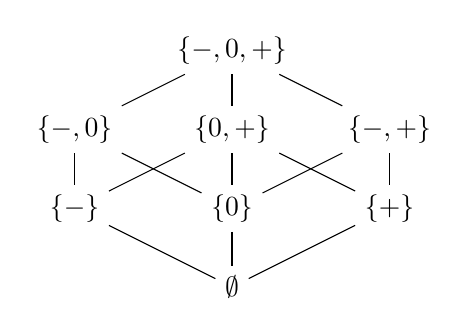
\begin{tikzpicture}
   \tikzstyle{line} = [draw, -latex'] 
   \node (nzp) at (2,3)  {$\{-,0,+\}$};
   \node (nz) at (0,2)  {$\{-,0\}$};
   \node (zp) at (2,2)  {$\{0,+\}$};
   \node (np) at (4,2)  {$\{-,+\}$};
   \node (n) at (0,1)  {$\{-\}$};
   \node (z) at (2,1)  {$\{0\}$};
   \node (p) at (4,1)  {$\{+\}$};
   \node (empty) at (2,0)  {$\emptyset$};
 
   \path [-] (nzp) edge (nz);
   \path [-] (nzp) edge  (np);
   \path [-] (nzp) edge  (zp);
 
   \path [-] (nz) edge (z);
   \path [-] (nz) edge (n);

   \path [-] (zp) edge (n);
   \path [-] (zp) edge (z);
   \path [-] (zp) edge (p);

   \path [-] (np) edge (z);
   \path [-] (np) edge (p);

   \path [-] (n) edge (empty);
   \path [-] (z) edge (empty);
   \path [-] (p) edge (empty);

 \end{tikzpicture}
  \caption{Complete lattice of sign detection instance}
 
  \label{fig:sign_detection_complete_lattice}
 \end{figure}
\noindent The top of the lattice gives the least precise solution and the bottom the most precise.
\\\\
We define the mapping of labels to transfer functions for the analysis in table~\ref{table:sign_detection_functions}.
\begin{table}[h]
\begin{tabular}{| l | l |}
  \hline
  Statement & Function \\
  \hline
  \hline
  [x := a]$^\ell$ & f$_\ell^S (\widehat{\sigma}) = \widehat{\sigma}[x \mapsto \mathcal{A}_S[\![a]\!] \widehat{\sigma} ]$ \\
  \hline
 [skip]$^\ell$ & f$_\ell^S (\widehat{\sigma}) = \widehat{\sigma}$\\
  \hline
 [b]$^\ell$ & f$_\ell^S (\widehat{\sigma}) = \widehat{\sigma}$\\
  \hline
  [int A[a$_1$] := a$_2$]$^\ell$ & f$_\ell^S (\widehat{\sigma}) = 
     \begin{cases} 
        \widehat{\sigma}[$A[a$_1$]$ \mapsto \bot]        & \text{if } \mathcal{A}_S [\![a_1]\!] \widehat{a} = \{-\} \\
        \widehat{\sigma}[$A[a$_1$]$ \mapsto A_I[\![a_2]\!] & \text{if }\mathcal{A}_S [\![a_1]\!] \widehat{a} \subseteq \{0,+\} \\
     \end{cases}$\\
  \hline
  [read x]$^\ell$ & f$_\ell^S (\widehat{\sigma}) = [x \mapsto \mathcal{A}_S [\![n]\!] \widehat{\sigma}]$ \\
  \hline
  [read A[a]]$^\ell$ & f$_\ell^S (\widehat{\sigma}) = 
     \begin{cases} 
        \widehat{\sigma}[$A[a]$ \mapsto \bot]        & \text{if } \mathcal{A}_S [\![a]\!]\widehat{\sigma} = \{-\} \\
        \widehat{\sigma}[$A[a]$ \mapsto \mathcal{A}_S[\![n]\!]\widehat{\sigma} & \text{if } \mathcal{A}_S [\![a]\!]\widehat{\sigma} = \{0,+\} \\
     \end{cases}$\\
  \hline
  [write A[n]]$^\ell$ & f$_\ell^S (\widehat{\sigma}) = \widehat{\sigma}$\\
  \hline
\end{tabular}
\centering
\caption{Transfer functions for sign detection}
\label{table:sign_detection_functions}
\end{table}

\subsection{Determine signs}
For the analysis to work the signs need to be determined for a given program. This is done by evaluating arithmetic expressions and boolean expressions.

\subsubsection{Evaluate arithmetic expressions}
In order to determine the sign of an expression we need to define the semantics of expressions in the \texttt{WHILE} language for the signs analysis.
$\mathcal{A}_S [\![a]\!]: \widehat{\textbf{State}_S} \rightarrow \textbf{Sign}$\\
We have the following monotone functions:\\
$\mathcal{A}_S [\![x]\!]\widehat{\sigma} = \widehat{\sigma} (x)\\
\mathcal{A}_S [\![n]\!]= 
   \begin{cases} 
      \{-\} & \text{ if } n < 0 \\
      \{0\} & \text{ if } n = 0 \\
      \{+\} & \text{ if } n > 0 \\
   \end{cases}\\
\mathcal{A}_S [\![a_1 \text{ op}_A a_2 ]\!] = \mathcal{A}_S [\![a_1]\!] \widehat{\sigma} \widehat{\text{ op}_A} \mathcal{A}_S [\![a_2]\!] \widehat{\sigma}, \text{where} \widehat{\text{ op}_A} : \textbf{Sign} \times \textbf{Sign} \rightarrow \textbf{Sign} \text{ is given by}:\\
\widehat{\text{ op}_A} (S_1, S_2) = \{ s_1 \text{ op}_A s_2 | s_1 \in S_1, s_2 \in S_2\}\\
\widehat{\text{ op}_A} \text {is a specific arithmetic operator from the set op}_a \{+,-,*,/\}.
$\\
Table~\ref{table:arithmetic_plus}, \ref{table:arithmetic_minus}, \ref{table:arithmetic_multiply}, \ref{table:arithmetic_division} define each of the operators.

\begin{table}[h]
\begin{tabular}{| r | c | c | c |}
\hline
 +   & -           & 0 & + \\
\hline
 -  & $\{-\}$     & $\{-\}$ & $\{-,0,+\}$ \\
\hline
 0  & $\{-\}$     & $\{0\}$ & $\{+\}$ \\
\hline
 +  & $\{-,0,+\}$ & $\{+\}$ & $\{+\}$ \\
\hline
\end{tabular}
\centering
\caption{Addition effects on variable state}
\label{table:arithmetic_plus}
\end{table}

\begin{table}[h]
\begin{tabular}{| r | c | c | c |}
\hline
  -  & -           & 0 & + \\
\hline
 -  & $\{-,0,+\}$ & $\{-\}$ & $\{-\}$ \\
\hline
 0  & $\{-\}$     & $\{0\}$ & $\{-\}$ \\
\hline
 +  & $\{+\}$     & $\{+\}$ & $\{-,0,+\}$ \\
\hline
\end{tabular}
\centering
\caption{Subtraction effects on variable state}
\label{table:arithmetic_minus}
\end{table}

\begin{table}[h]
\begin{tabular}{| r | c | c | c |}
\hline
 x   & -           & 0 & + \\
\hline
 -  & $\{+\}$ & $\{0\}$ & $\{-\}$ \\
\hline
 0  & $\{0\}$ & $\{0\}$ & $\{0\}$ \\
\hline
 +  & $\{-\}$ & $\{0\}$ & $\{+\}$ \\
\hline
\end{tabular}
\centering
\caption{Multiplication effects on variable state}
\label{table:arithmetic_multiply}
\end{table}

\begin{table}[h]
\begin{tabular}{| r | c | c | c |}
\hline
 \textbackslash   & -           & 0 & + \\
\hline
 -  & $\{+\}$ & $\emptyset$ & $\{-\}$ \\
\hline
 0  & $\{0\}$ & $\emptyset$ & $\{0\}$ \\
\hline
 +  & $\{-\}$ & $\emptyset$ & $\{+\}$ \\
\hline
\end{tabular}
\centering
\caption{Division effects on variable state}
\label{table:arithmetic_division}
\end{table}

\subsubsection{Evaluate boolean expressions}
Similarly booleans expressions should be evaluated. We that that:\\
$BExp \rightarrow \widehat{\textbf{State}_S} \rightarrow \textbf{P(\{tt,ff\})}$ which will be given by:\\
$\mathcal{B}_S [\![a_1op_ra_2]\!]\widehat{\sigma}' = \mathcal{A}_S [\![a_1]\!]\widehat{\sigma}'\widehat{op_r}\mathcal{A}_S [\![a_2]\!]\widehat{\sigma}'$\\
$\mathcal{B}_S [\![a_1op_ba_2]\!]\widehat{\sigma}' = \mathcal{B}_S [\![b_1]\!]\widehat{\sigma}'\widehat{op_b}\mathcal{B}_S [\![b_2]\!]\widehat{\sigma}'$\\
$\mathcal{B}_S [\![\neg b]\!]\widehat{\sigma}' =\{\neg t|t\in \mathcal{B}_S[\![b]\!]\widehat{\sigma}'\}$\\
\\
Where $\widehat{\text{op}_r}$ is a specific  operator from the set op$_r$ \{ $\leq,\geq,\neq,=,>,<$ \}, and where $\widehat{\text{op}_b}$ is a specific operator from the set op$_b$ \{$\&,|\}$.

\begin{table}
\begin{tabular}{| r | c | c |}
\hline
 \&   & tt   & ff  \\
\hline
 tt  & $\{tt\}$ & $\{ff\}$  \\
\hline
 ff  & $\{ff\}$ & $\{ff\}$ \\
\hline
\end{tabular}
\centering
\caption{Possible outcomes of AND operator.}
\label{table:and_operator}
\end{table}

\begin{table}
\begin{tabular}{| r | c | c |}
\hline
 |   & tt   & ff  \\
\hline
 tt  & $\{tt\}$ & $\{ff\}$  \\
\hline
 ff  & $\{tt\}$ & $\{ff\}$ \\
\hline
\end{tabular}
\centering
\caption{Possible outcomes of OR operator.}
\label{table:or_operator}
\end{table}

\begin{table}
\begin{tabular}{| r | c | c | c |}
\hline
 <   & -   & 0 & +  \\
\hline
 -  & $\{tt,ff\}$ & $\{tt\}$ & $\{tt\}$  \\
\hline
 0  & $\{ff\}$ & $\{ff\}$ & $\{tt\}$ \\
\hline
 +  & $\{ff\}$ & $\{ff\}$ & $\{tt,ff\}$ \\
 \hline
\end{tabular}
\centering
\caption{Possible outcomes of < operator.}
\label{table:less_than_operator}
\end{table}

\begin{table}
\begin{tabular}{| r | c | c | c |}
\hline
 >   & -   & 0 & +  \\
\hline
 -  & $\{tt,ff\}$ & $\{ff\}$ & $\{ff\}$  \\
\hline
 0  & $\{tt\}$ & $\{ff\}$ & $\{ff\}$ \\
\hline
 +  & $\{tt\}$ & $\{tt\}$ & $\{tt,ff\}$ \\
 \hline
\end{tabular}
\centering
\caption{Possible outcomes of > operator.}
\label{table:greater_than_operator}
\end{table}

\begin{table}
\begin{tabular}{| r | c | c | c |}
\hline
 $\leq$   & -   & 0 & +  \\
\hline
 -  & $\{tt,ff\}$ & $\{tt\}$ & $\{tt\}$  \\
\hline
 0  & $\{ff\}$ & $\{tt\}$ & $\{tt\}$ \\
\hline
 +  & $\{ff\}$ & $\{ff\}$ & $\{tt,ff\}$ \\
 \hline
\end{tabular}
\centering
\caption{Possible outcomes of $\leq$ operator.}
\label{table:less_than_equal_operator}
\end{table}

\begin{table}
\begin{tabular}{| r | c | c | c |}
\hline
 $\geq$   & -   & 0 & +  \\
\hline
 -  & $\{tt,ff\}$ & $\{ff\}$ & $\{ff\}$  \\
\hline
 0  & $\{tt\}$ & $\{tt\}$ & $\{ff\}$ \\
\hline
 +  & $\{tt\}$ & $\{tt\}$ & $\{tt,ff\}$ \\
 \hline
\end{tabular}
\centering
\caption{Possible outcomes of $\geq$ operator.}
\label{table:greater_than_equal_operator}
\end{table}

\begin{table}
\begin{tabular}{| r | c | c | c |}
\hline
 $=$   & -   & 0 & +  \\
\hline
 -  & $\{tt,ff\}$ & $\{ff\}$ & $\{ff\}$  \\
\hline
 0  & $\{ff\}$ & $\{tt\}$ & $\{ff\}$ \\
\hline
 +  & $\{ff\}$ & $\{ff\}$ & $\{tt,ff\}$ \\
 \hline
\end{tabular}
\centering
\caption{Possible outcomes of $=$ operator.}
\label{table:equal_operator}
\end{table}

\begin{table}
\begin{tabular}{| r | c | c | c |}
\hline
 $\neq$   & -   & 0 & +  \\
\hline
 -  & $\{tt,ff\}$ & $\{tt\}$ & $\{tt\}$  \\
\hline
 0  & $\{tt\}$ & $\{ff\}$ & $\{tt\}$ \\
\hline
 +  & $\{tt\}$ & $\{tt\}$ & $\{tt,ff\}$ \\
 \hline
\end{tabular}
\centering
\caption{Possible outcomes of $=$ operator.}
\label{table:not_equal_operator}
\end{table}


\subsection{Lower bound detection}
Check for an assignment which includes an operation with an array, that the sign of the array is not $\emptyset$. If so, we know that the index parameter is invalid according to the lower bounds.

\subsection{Constraints}
\begin{table}[H]
\begin{tabular}{| l | l |}
\hline
A$_\circ (1) = \iota \{\text{init}(S_*) \} $ & A$_\bullet(1) = \text{f}_{\text{int A[2]}} (\text{A}_\circ (1))$ \\
\hline
A$_\circ (2) =$A$_\bullet(1) $ & A$_\bullet(2) = \text{f}_{\text{int i}} (\text{A}_\circ (2))$ \\
\hline
A$_\circ (3) = $A$_\bullet(2)$ & A$_\bullet(3) = \text{f}_{\text{i := -1}} (\text{A}_\circ (3))$  \\
\hline
A$_\circ (4) = $A$_\bullet(3) \bigcup $A$_\bullet(6) $ & A$_\bullet(4) = \text{f}_{\text{i < 3}} (\text{A}_\circ (4))$ \\
\hline
A$_\circ (5) = $A$_\bullet(4)$ & A$_\bullet(5) = \text{f}_{\text{A[i] := i + 1}} (\text{A}_\circ (5))$ \\
\hline
A$_\circ (6) = $A$_\bullet(5)$ & A$_\bullet(6) = \text{f}_{\text{i := i + 1}} (\text{A}_\circ (6))$ \\

\hline
\end{tabular}
\centering
\end{table}

\begin{table}[H]
\begin{tabular}{| r | c | c | c |}
\hline
A$_\bullet (\cdot) $ & A[0]        & A[1]        & i \\
\hline
1                    & $\{0\}$     & $\{0\} $    & $\emptyset$ \\
2                    & $\{0\}$     & $\{0\} $    & $\{0\}$ \\
3                    & $\{0\}$     & $\{0\} $    & $\{-\}$ \\
4                    & $\{-,0,+\}$ & $\{-,0,+\}$ & $\{-,0,+\}$ \\
5                    & $\{-,0,+\}$ & $\{-,0,+\}$ & $\{-,0,+\}$ \\
6                    & $\{-,0,+\}$ & $\{-,0,+\}$ & $\{-,0,+\}$ \\
\hline
\end{tabular}
\centering
\end{table}
